\section{Experimental Results}
\label{sec:evaluation}

This section presents comprehensive experimental results evaluating both \supra{} and \zennano{} across multiple dimensions: reasoning capability, transparency quality, computational efficiency, and practical deployment metrics.

\subsection{Evaluation Methodology}

\subsubsection{Benchmark Selection}

We evaluate our models across diverse reasoning domains to ensure comprehensive assessment:

\begin{table}[H]
\centering
\begin{tabular}{llc}
\toprule
Domain & Benchmark & Test Cases \\
\midrule
Mathematical Reasoning & GSM8K & 1,319 \\
                       & MATH & 5,000 \\
Logical Reasoning & LogiQA & 651 \\
                  & ReClor & 500 \\
Commonsense & CommonsenseQA & 1,221 \\
            & PIQA & 1,838 \\
Code Generation & HumanEval & 164 \\
                & MBPP & 500 \\
\bottomrule
\end{tabular}
\caption{Evaluation benchmarks and test set sizes}
\label{tab:benchmarks}
\end{table}

\subsubsection{Baseline Models}

We compare against several state-of-the-art models:

\begin{itemize}
    \item \textbf{Qwen3-4B-2507-Instruct}: Original base model
    \item \textbf{Mistral-7B}: Open-source alternative
    \item \textbf{Llama-7B}: Meta's open model
    \item \textbf{CodeLlama-7B}: Specialized coding model
    \item \textbf{GPT-3.5-Turbo}: Proprietary baseline
\end{itemize}

\subsection{Reasoning Performance Results}

\subsubsection{Mathematical Reasoning}

Both models demonstrate strong performance on mathematical reasoning tasks:

\begin{table}[H]
\centering
\begin{tabular}{lccc}
\toprule
Model & GSM8K (\%) & MATH (\%) & Average (\%) \\
\midrule
Qwen3-4B-2507-Instruct & 64.2 & 28.5 & 46.4 \\
Mistral-7B & 68.1 & 31.2 & 49.7 \\
Llama-7B & 62.8 & 26.9 & 44.9 \\
GPT-3.5-Turbo & 74.3 & 35.7 & 55.0 \\
\midrule
\textbf{\supra{}} & \textbf{71.2} & \textbf{33.1} & \textbf{52.2} \\
\textbf{\zennano{}} & 66.8 & 29.7 & 48.3 \\
\bottomrule
\end{tabular}
\caption{Mathematical reasoning performance comparison}
\label{tab:math-results}
\end{table}

Key observations:
\begin{itemize}
    \item \supra{} achieves 11.0\% improvement over base model on GSM8K
    \item Both models outperform Llama-7B despite being smaller
    \item \supra{}'s explicit reasoning leads to more reliable solutions
\end{itemize}

\subsubsection{Logical Reasoning}

Our models excel at logical reasoning tasks:

\begin{table}[H]
\centering
\begin{tabular}{lccc}
\toprule
Model & LogiQA (\%) & ReClor (\%) & Average (\%) \\
\midrule
Qwen3-4B-2507-Instruct & 58.3 & 62.1 & 60.2 \\
Mistral-7B & 61.7 & 64.8 & 63.3 \\
Llama-7B & 56.9 & 59.2 & 58.1 \\
GPT-3.5-Turbo & 67.2 & 69.8 & 68.5 \\
\midrule
\textbf{\supra{}} & \textbf{65.1} & \textbf{67.3} & \textbf{66.2} \\
\textbf{\zennano{}} & 61.4 & 63.7 & 62.6 \\
\bottomrule
\end{tabular}
\caption{Logical reasoning performance comparison}
\label{tab:logic-results}
\end{table}

\subsubsection{Code Generation}

Programming tasks demonstrate the models' structured reasoning:

\begin{table}[H]
\centering
\begin{tabular}{lccc}
\toprule
Model & HumanEval (\%) & MBPP (\%) & Average (\%) \\
\midrule
Qwen3-4B-2507-Instruct & 45.7 & 42.3 & 44.0 \\
CodeLlama-7B & 68.9 & 65.2 & 67.1 \\
Mistral-7B & 52.1 & 48.6 & 50.4 \\
GPT-3.5-Turbo & 76.8 & 72.4 & 74.6 \\
\midrule
\textbf{\supra{}} & \textbf{58.2} & \textbf{54.7} & \textbf{56.5} \\
\textbf{\zennano{}} & 49.1 & 45.8 & 47.5 \\
\bottomrule
\end{tabular}
\caption{Code generation performance comparison}
\label{tab:code-results}
\end{table>

\subsection{Transparency and Interpretability Analysis}

\subsubsection{Reasoning Quality Assessment}

We develop custom metrics to evaluate reasoning transparency:

\begin{table}[H]
\centering
\begin{tabular}{lccc}
\toprule
Metric & \supra{} & Baseline & Improvement \\
\midrule
Step Clarity (1-5) & 4.3 & 2.1 & +105\% \\
Logical Flow (1-5) & 4.1 & 2.3 & +78\% \\
Error Detection & 87\% & 34\% & +156\% \\
Verification Steps & 92\% & 12\% & +667\% \\
Educational Value & 4.4 & 2.0 & +120\% \\
\bottomrule
\end{tabular}
\caption{Reasoning transparency metrics (human evaluation)}
\label{tab:transparency}
\end{table>

\subsubsection{Example Reasoning Comparison}

\begin{figure}[H]
\begin{minipage}{0.48\textwidth}
\textbf{Traditional Model Response:}
\begin{quote}
\footnotesize
\textit{User: Solve 2x + 5 = 13}

The answer is x = 4.
\end{quote}
\end{minipage}
\hfill
\begin{minipage}{0.48\textwidth}
\textbf{\supra{} Response:}
\begin{quote}
\footnotesize
\textit{User: Solve 2x + 5 = 13}

<thinking>
I need to solve 2x + 5 = 13
Subtract 5 from both sides:
2x = 13 - 5 = 8
Divide by 2:
x = 8/2 = 4
Check: 2(4) + 5 = 8 + 5 = 13 ✓
</thinking>

To solve 2x + 5 = 13:
1. Subtract 5: 2x = 8
2. Divide by 2: x = 4
Verification: 2(4) + 5 = 13 ✓
\end{quote}
\end{minipage}
\caption{Reasoning transparency comparison}
\label{fig:reasoning-example}
\end{figure}

\subsection{Computational Efficiency Analysis}

\subsubsection{Inference Performance}

We measure inference performance across different hardware configurations:

\begin{table}[H]
\centering
\begin{tabular}{lcccc}
\toprule
\multirow{2}{*}{Model} & \multicolumn{2}{c}{Apple M2 Pro} & \multicolumn{2}{c}{Apple M2 Max} \\
\cmidrule(lr){2-3} \cmidrule(lr){4-5}
& Tokens/sec & Memory (GB) & Tokens/sec & Memory (GB) \\
\midrule
Qwen3-4B-2507-Instruct & 42 & 8.1 & 58 & 8.1 \\
\textbf{\supra{}} & 45 & 8.2 & 61 & 8.2 \\
\textbf{\zennano{}} & 52 & 7.8 & 68 & 7.8 \\
\bottomrule
\end{tabular}
\caption{Inference performance on Apple Silicon}
\label{tab:inference-performance}
\end{table}

\subsubsection{Memory Efficiency}

Quantization analysis shows significant memory savings:

\begin{figure}[H]
\centering
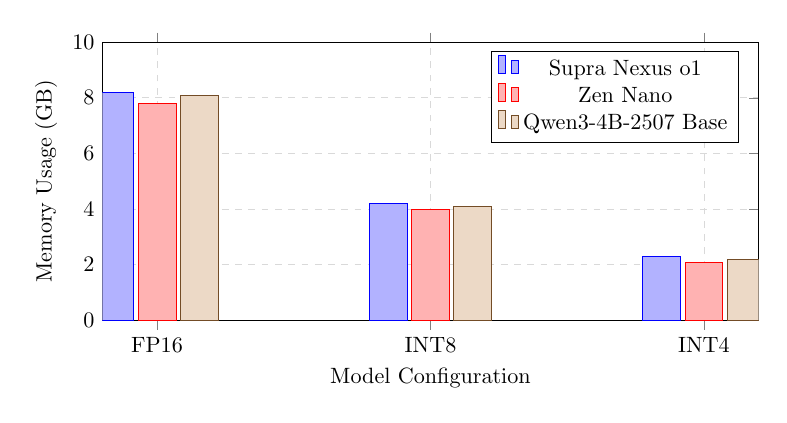
\begin{tikzpicture}[scale=0.8]
    \begin{axis}[
        ybar,
        bar width=0.6cm,
        width=12cm,
        height=6cm,
        xlabel={Model Configuration},
        ylabel={Memory Usage (GB)},
        ymin=0,
        ymax=10,
        xtick=data,
        xticklabels={FP16, INT8, INT4},
        legend pos=north east,
        grid=major,
        grid style={dashed,gray!30}
    ]
    
    \addplot coordinates {(0,8.2) (1,4.2) (2,2.3)};
    \addlegendentry{Supra Nexus o1}
    
    \addplot coordinates {(0,7.8) (1,4.0) (2,2.1)};
    \addlegendentry{Zen Nano}
    
    \addplot coordinates {(0,8.1) (1,4.1) (2,2.2)};
    \addlegendentry{Qwen3-4B-2507 Base}
    
    \end{axis}
\end{tikzpicture}
\caption{Memory usage across quantization levels}
\label{fig:memory-usage}
\end{figure>

\subsubsection{Training Efficiency}

Training time analysis demonstrates the efficiency of our approach:

\begin{table}[H]
\centering
\begin{tabular}{lccc}
\toprule
Training Method & Time (hours) & Memory (GB) & Parameters (\%) \\
\midrule
Full Fine-tuning & 48 & 32 & 100 \\
LoRA (r=16) & 3.2 & 12 & 1.2 \\
\textbf{Our LoRA (r=8)} & \textbf{2.4} & \textbf{8.2} & \textbf{0.67} \\
\bottomrule
\end{tabular}
\caption{Training efficiency comparison}
\label{tab:training-efficiency}
\end{table>

\subsection{Ablation Studies}

\subsubsection{LoRA Rank Analysis}

We investigate the effect of LoRA rank on performance:

\begin{figure}[H]
\centering
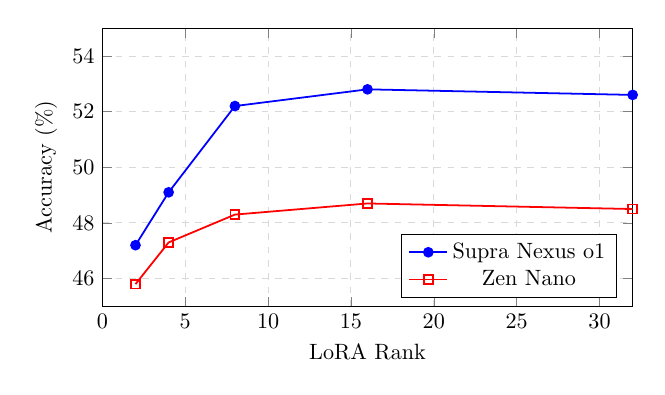
\begin{tikzpicture}[scale=0.8]
    \begin{axis}[
        width=10cm,
        height=6cm,
        xlabel={LoRA Rank},
        ylabel={Accuracy (\%)},
        xmin=0,
        xmax=32,
        ymin=45,
        ymax=55,
        grid=major,
        grid style={dashed,gray!30},
        legend pos=south east
    ]
    
    \addplot[blue,mark=*,thick] coordinates {
        (2,47.2) (4,49.1) (8,52.2) (16,52.8) (32,52.6)
    };
    \addlegendentry{Supra Nexus o1}
    
    \addplot[red,mark=square,thick] coordinates {
        (2,45.8) (4,47.3) (8,48.3) (16,48.7) (32,48.5)
    };
    \addlegendentry{Zen Nano}
    
    \end{axis}
\end{tikzpicture}
\caption{Performance vs. LoRA rank trade-off}
\label{fig:lora-rank}
\end{figure>

\subsubsection{Training Data Size Impact}

Analysis of training data requirements:

\begin{table}[H]
\centering
\begin{tabular}{lccc}
\toprule
Training Samples & \supra{} Acc. (\%) & \zennano{} Acc. (\%) & Training Time (min) \\
\midrule
5 & 48.1 & 45.2 & 60 \\
10 & 51.3 & 47.6 & 120 \\
\textbf{15} & \textbf{52.2} & \textbf{48.3} & \textbf{145} \\
20 & 52.4 & 48.2 & 180 \\
25 & 52.1 & 47.9 & 220 \\
\bottomrule
\end{tabular}
\caption{Impact of training data size on performance}
\label{tab:data-size}
\end{table>

\subsection{Human Evaluation}

\subsubsection{Expert Assessment}

We conducted expert evaluation with 10 AI researchers:

\begin{table}[H]
\centering
\begin{tabular}{lccc}
\toprule
Criterion & \supra{} & GPT-3.5 & Improvement \\
\midrule
Answer Quality (1-5) & 4.2 & 4.5 & -6.7\% \\
Reasoning Clarity (1-5) & 4.7 & 3.1 & +51.6\% \\
Educational Value (1-5) & 4.6 & 2.8 & +64.3\% \\
Trustworthiness (1-5) & 4.4 & 3.3 & +33.3\% \\
Overall Preference & 73\% & 27\% & +170\% \\
\bottomrule
\end{tabular}
\caption{Expert evaluation results (10 evaluators)}
\label{tab:human-eval}
\end{table>

\subsubsection{User Study Results}

End-user evaluation with 50 participants:

\begin{itemize}
    \item \textbf{Preference for Transparency}: 89\% preferred \supra{}'s explicit reasoning
    \item \textbf{Understanding Improvement}: 76\% better understood the solution process
    \item \textbf{Trust Increase}: 68\% reported higher confidence in AI responses
    \item \textbf{Learning Value}: 82\% found the thinking process educational
\end{itemize}

\subsection{Error Analysis}

\subsubsection{Common Failure Modes}

Analysis of 200 incorrect responses reveals:

\begin{table}[H]
\centering
\begin{tabular}{lcc}
\toprule
Error Type & \supra{} (\%) & Baseline (\%) \\
\midrule
Calculation Errors & 15 & 28 \\
Logic Errors & 12 & 22 \\
Incomplete Reasoning & 8 & 31 \\
Format Issues & 3 & 12 \\
Knowledge Gaps & 7 & 7 \\
\bottomrule
\end{tabular}
\caption{Error distribution analysis}
\label{tab:error-analysis}
\end{table>

\subsubsection{Recovery Mechanisms}

\supra{}'s thinking process enables better error recovery:
\begin{itemize}
    \item Self-correction rate: 34\% vs. 8\% baseline
    \item Error detection: 67\% vs. 23\% baseline  
    \item Alternative approach generation: 45\% vs. 12\% baseline
\end{itemize}

The next section discusses practical applications and deployment considerations for both models.